\anonsection{Задание 11}
\anonsubsection{Формулировка задания}
Построить двумерное пуассоновское поле, отвечающее сложному 
 пуассоновскому процессу:

\begin{enumerate}
	\item Первая интерпретация: система массового обслуживания. При этом 
     первая координата поля~---~время поступления заявки в СМО 
     (равномерное распределение), вторая~---~время её обслуживания 
     (распределение \( \chi^2 \) с \( 10 \)-ю степенями свободы).
	
	\item Вторая интерпретация: система массового обслуживания с 
     циклической интенсивностью \( \lambda(t)=\lambda_0(1+\cos(t)) \) и 
     единичными скачками. Свести данную задачу моделирования 
     неоднородного пуассоновского процесса при помощи метода Льюиса и 
     Шедлера к моделированию двумерного пуассоновского поля, где первая 
     координата имеет равномерное распределение, а вторая~---~распределение 
     Бернулли.
	
	\item Третья интерпретация: работа страховой компании. Первая 
     координата~---~момент наступления страхового случая (равномерное 
     распределение), вторая координата~---~величина ущерба (распределение 
     Парето). Поступление капитала по времени линейно со скоростью 
     \( c>0 \), начальный капитал \( W>0 \).
	
	\item Для каждой системы рассмотреть всевозможные случаи поведения 
     системы в зависимости от значения параметров.
	
\end{enumerate}




\anonsubsection{Первая интерпретация: система массового обслуживания}
Пусть $\lambda$ --- интенсивность пуассоновского поля. Времена 
 поступления заявок генерируются так, что $\Delta t_i = t_i - t_{i - 1} 
 \sim Exp(\lambda)$.
 Время обслуживания каждой заявки $s_i$ независимы и генерируются как 
 случайные величины с распределением $\chi^2(10)$.\\
Поскольку все заявки обрабатываются последовательно, время окончания 
 обработки заявки, поступившей в момент времени $t_i$ можно найти 
 следующим образом:
\begin{itemize}
	\item если к моменту поступления заявки предыдущая заявка уже 
     обработана, то нужно к времени поступления текущей заявки прибавить 
     время ее обработки;
	\begin{center}
		$Q_i = t_i + s_i.$
	\end{center}
	\item если предыдущая заявка еще не обработана, то нужно прибавить к 
     времени конца обработки предыдущей заявки время обработки текущей.
\begin{center}
		$Q_i = Q_{i-1} + s_i.$
\end{center}

\end{itemize}
Обобщая вышесказанное, имеем:
\begin{center}
		$Q_i = t_i + \max(0, Q_{i - 1} - t_i) + s_i.$
\end{center}

Для каждой заявки будем считать количество людей в очереди.

\begin{itemize}
	\item если во время поступления $i$-й заявки очереди не было, то 
     положим $n_i = 0$.

	\item если предыдущая заявка еще не обработана, то 
	
	\begin{center}
		$n_i \neq Q_k : k < i$ и $Q_k > t_i$
	\end{center}
т. е. количество еще не выполненных к моменту времени $t_i$ заявок.
\end{itemize}

Поскольку время обработки одной заявки в среднем равно 10, а средний 
 интервал между поступлениями заявок равен $\mathbb{E}\Delta_i = 
 \frac{1}{\lambda}$, то при $\lambda < 0.1$ очереди практически не 
 будет, а при $\lambda > 0.1$ очередь будет неограниченно расти. Этот
 эффект продемонстрирован на Рис.\eqref{fig:queuing}.

\begin{figure}[ht]
    \centering
    \begin{subfigure}[b]{0.49\textwidth}
        \centering
        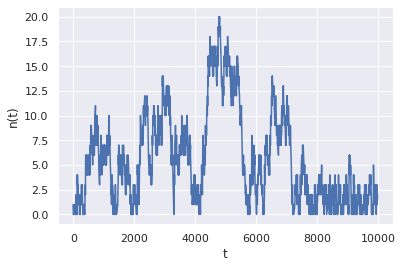
\includegraphics[width=\textwidth]{./resources/queuing_0.09.png}
        \caption{Моделирование очереди при $ \lambda = 0.09 $. Система 
         справляется.}
        \label{subfig:queuing_0.09}
    \end{subfigure}
    \hfill
    \begin{subfigure}[b]{0.49\textwidth}
        \centering
        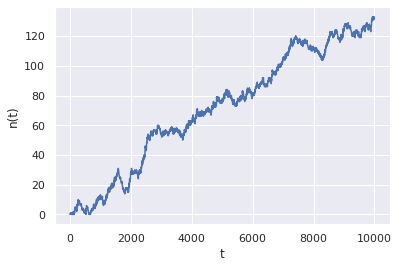
\includegraphics[width=\textwidth]{./resources/queuing_0.11.png}
        \caption{Моделирование очереди при $ \lambda = 0.11 $. Очередь 
         растет.}
        \label{subfig:queuing_0.11}
    \end{subfigure}
    \caption{Моделирование очереди при разных показателях интенсивности.}
    \label{fig:queuing}
\end{figure}

\anonsubsection{Вторая интерпретация: система массового обслуживания с 
циклической интенсивностью  и единичными скачками}


Пусть \( T_1,\ldots,T_n,\ldots \)~---~времена наступления некоторых 
 событий, а \( N(t_1,t_2) \)~---~количество событий, произошедших в 
 промежуток \( [t_1,t_2] \). Заметим, что \( T_{n+1}-T_n \) имеет 
 функцию распределения \( F(x)=1-e^{-(\Lambda(t+x)-\Lambda(t))}, x 
 \geq 0 \), где 


\[
 \Lambda(t)=\int\limits_0^t\lambda(u)du=\lambda(t+\sin t).
\]
неограниченно возрастает с ростом \( t \). 

\( T_{n+1} \) распределено как \( T_n+F^{-1}(U) \), где \( U \) 
 равномерно распределена на \( [0,1] \). Заметим, что если записать 
 \( U \) как \( 1-e^{-E} \), где \( E \)~---~экспоненциальная случайная 
 величина с параметром \( \lambda_E=1 \), то \( T_{n+1} \) распределена 
 как \( \Lambda^{-1}(E+\Lambda(T_n)) \).

Будем искать обратную функцию \( \Lambda^{-1}(y) \) численно, так как 
 аналитически это не представляется возможным ( \( \Lambda'(t) = 
 \lambda_0(1+\cos(t)) \)) почти всюду положительна, то есть функция 
 возрастает). Такой метод моделирования неоднородного процесса Пуассона 
 называется методом Льюиса--Шедлера.

Чтобы не искать обратную функцию, можно воспользоваться следующей 
 модификацией метода Льюиса--Шедлера. Пусть имеется переменная \( t \), 
 в которой хранится текущее время (но не обязательно событие произошло 
 строго в это время). 

\begin{itemize}
	\item На каждом шаге генерируем случайную величину \( \xi \sim 
     \Exp(2\lambda_0) \).
	\item Прибавляем к переменной \( t \) величину \( \xi \) и генерируем 
     случайную величину \( \eta=\Bern((1+\cos t)/2) \).
	\begin{itemize}
			\item если она приняла значение \( 1 \), то полагаем 
             \( T_{i+1}=t \) и \( i=i+1 \)
			\item иначе ничего не делаем и повторяем процесс заново
	\end{itemize}
\end{itemize}

На Рис.\eqref{fig:queuing_cycling} изображена смоделированная система с 
 циклической интенсивностью. Промежуткам роста длины очереди соответсвуют
 промежутки возрастания интенсивности.
\begin{figure}[ht]
	\centering
	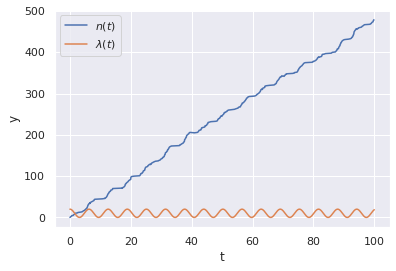
\includegraphics[width = 0.7\linewidth]{"./resources/queuing_cycling.png"}
	\caption{Система массового обслуживания с циклической интенсивностью.}
    \label{fig:queuing_cycling}
\end{figure}

\anonsubsection{Третья интерпретация: работа страховой компании.}
\begin{definition}
	Случайная величина $X$ имеет распределение Парето с параметрами 
     $x_m$ и $k$, если ее функция распределения имеет вид:
	\begin{equation*}
	F_X(x) = 1 - \left(\frac{x_m}{x}\right)^k.
	\end{equation*}
\end{definition}
Для моделирования случайной величины, имеющей распределение Парето, 
 снова воспользуемся методом обратной функции.\\
Обратная функция для данной функции распределения имеет вид:
\begin{equation}
F_X^{-1}(x) = \frac{x_m}{(1 - x)^{\frac{1}{k}}}.
\end{equation}

Сгенерируем времена наступления страховых случаев на временном интервале 
 \( [0,T] \):
\[
0 \leq t_1 \leq t_2 \leq \ldots \leq t_n \leq T,
\]
причём \( t_i-t_{i-1} \sim \Exp(\lambda) \), \( \lambda>0 \)~---~интенсивность 
 потока страховых случаев.

Величину ущерба \( s_i \) страхового случая в момент времени \( t \) 
 будем генерировать с помощью распределения Парето с параметрами 
 \( x_m \) и \( k \). Случайную величину, распределённую по Парето, 
 будем генерировать, воспользовавшись методом обратных функций:
\[
F_{\xi}^{-1}(y)=\dfrac{x_m}{\left(1-x\right)^{\frac{1}{k}}}.
\]

Учтем, что если \( Y\sim U[0,1] \), то и \( (1-Y)\sim U[0,1] \). Тогда 
 случайная величина
\[
X=x_mY^{-\frac{1}{k}},\quad Y\sim U[0,1]
\]
имеет распределение Парето с параметрами \( x_m \) и \( k \).

Величина капитала компании в момент времени \( t \) выражается как
\[
W_t=W_0+ct-s(t),
\]
где \( s(t) \)~---~сумма величин ущерба страховых случаев, произошедших 
 в моменты времени \( t_i \) такие, что \( t_i\leqslant t \). Время 
 разорения~---~случайная величина, задаваемая следующим условием:
\[
T=\min\lbrace t>0|W_t<0\rbrace.
\]

Выведем зависимость функции \( W(t) \) от параметров \( \lambda \), 
 \( x_m \), \( k \), \( W_0 \), \( c \). Будем считать, что \( k>1 \). 
 Тогда
\[
\mathbb{E}W'(t)=c-\mathbb{E}'s(t)=c-\left(\mathbb{E}\left[\sum\limits_{t_i<t}
 s_i\right]\right)'=c-\left(\dfrac{t}{\frac{1}{\lambda}}\mathbb{E}[s_i]
 \right)'=c-\dfrac{\lambda kx_m}{k-1}.
\]

Таким образом,
\begin{itemize}
	\item при \( c(k-1)>\lambda k x_m \) капитал растёт
	\item при \( c(k-1)=\lambda k x_m \) система находится в положении 
     равновесия
	\item при \( c(k-1)<\lambda k x_m \) капитал уменьшается
\end{itemize}

На Рис.\eqref{fig:ins_comp} изображено уменьшение, баланс и рост капитала
 компании в зависимости от параметров.

\begin{figure}[ht]
    \centering
    \begin{subfigure}[b]{0.49\textwidth}
        \centering
        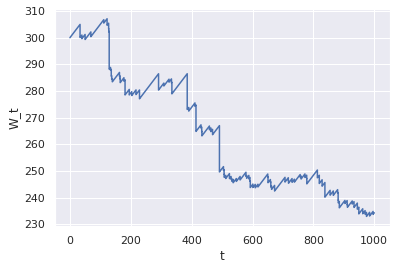
\includegraphics[width=\textwidth]{./resources/ins_comp_decreasing.png}
        \caption{Уменьшение капитала: $\lambda = 0.1, x_m = 1, k = 2, c = 0.15. $}
        \label{subfig:ins_comp_decreasing}
    \end{subfigure}
    \hfill
    \begin{subfigure}[b]{0.49\textwidth}
        \centering
        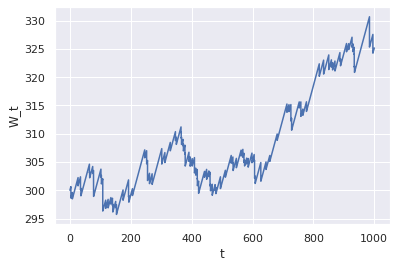
\includegraphics[width=\textwidth]{./resources/ins_comp_balancing.png}
        \caption{Баланс капитала: $\lambda = 0.1, x_m = 1, k = 2, c = 0.2. $}
        \label{subfig:ins_comp_balancing}
    \end{subfigure}
    \hfill
    \begin{subfigure}[b]{0.49\textwidth}
        \centering
        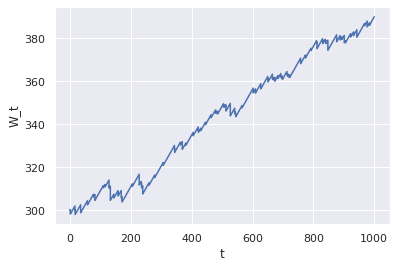
\includegraphics[width=\textwidth]{./resources/ins_comp_increasing.png}
        \caption{Увеличение капитала: $\lambda = 0.1, x_m = 1, k = 2, c = 0.25. $}
        \label{subfig:ins_comp_increasing}
    \end{subfigure}
    \caption{Моделирование капитала страховой компании.}
    \label{fig:ins_comp}
\end{figure}